\chapter{SYSTEM ARCHITECTURE}

\section{Introduction to System Design}

Securi Sphere employs a 3-layer SIEM pipeline architecture modeled after IBM QRadar, adapted for small Linux fleets. The architecture decouples data collection, processing, and search into distinct layers, enabling independent scaling and deployment. The platform comprises three primary components: Linux agents, a FastAPI backend, and a Next.js frontend dashboard, communicating via HTTPS/JSON and WebSocket protocols.

\section{Three-Layer SIEM Pipeline}

The system implements the following layered architecture:

\begin{center}
\begin{tikzpicture}[node distance=2cm, auto]
    % Layer 1: Collection
    \node [draw, rectangle, minimum width=3cm, minimum height=2cm, fill=blue!15] (L1) {Layer 1 — Collection};
    \node [draw, rectangle, minimum width=3cm, minimum height=2cm, fill=green!15, right=of L1] (L2) {Layer 2 — Processing};
    \node [draw, rectangle, minimum width=3cm, minimum height=2cm, fill=orange!15, right=of L2] (L3) {Layer 3 — Search};
    
    % Sub-nodes under Layer 1
    \node [below=of L1, xshift=-2cm] (agents) {Linux Agents};
    \node [below=of L1, xshift=2cm] (buffer) {Offline Buffer};
    
    % Connections
    \draw [->, thick] (agents) -- node {HMAC-signed HTTPS} (L1);
    \draw [->, thick] (L1) -- node {POST /api/v1/agent/events} (L2);
    \draw [->, thick] (buffer) -- node {auto-replay} (L2);
    \draw [->, thick] (L2) -- node {Redis pub/sub} (L3);
    \draw [->, thick] (L3) -- node {PostgreSQL + OpenSearch} (L2);
\end{tikzpicture}
\end{center}

\noindent\textbf{Layer 1 — Collection:} Linux agents running on target hosts collect system logs (auth.log, syslog, journald), CPU/memory/disk metrics via psutil, and network flow data. Events are batched every 10 seconds and transmitted via HTTPS with HMAC-SHA256 signing. Each agent maintains a SQLite offline buffer for local storage when network connectivity is unavailable; events are auto-replayed upon reconnection with exponential backoff on persistent failures.

\noindent\textbf{Layer 2 — Processing:} The ingestion pipeline performs four steps: (1) payload validation (batch size 1-100 events, timestamp bounds, string field limits), (2) event normalization (mapping variant names to canonical types, extracting source\_ip, username, category), (3) deduplication using SHA-256 fingerprinting with Redis SETEX fast path and PostgreSQL fallback, and (4) enrichment with MITRE ATT\&CK technique mapping and IOC matching, with storage to PostgreSQL and optional OpenSearch indexing.

\noindent\textbf{Layer 3 — Search:} The processing engine runs detection rules, correlation algorithms, and UEBA analysis. Detected alerts are grouped into offenses via the QRadar-style offense engine. Real-time updates are pushed to the frontend via Redis pub/sub/WebSocket. Analyst queries are executed via the /api/v1/siem and /api/v1/search endpoints, with OpenSearch enabling full-text search at scale.

\section{Component Map}

| Layer | Component | Code Location | Description |
|-------|-----------|---------------|-------------|
| \textbf{Collection} | Agent collectors | `agent/agent/collector/` | Log collection, metrics extraction, heartbeat |
| \textbf{Collection} | Offline buffer | `agent/agent/buffer.py` | SQLite local buffer, auto-replay on reconnect |
| \textbf{Collection} | HMAC signing | `agent/agent/sender.py` | Per-agent API key signing with nonce validation |
| \textbf{Gatekeeper} | Signature verification | `backend/app/services/agent_auth.py` | HMAC-SHA256 constant-time comparison |
| \textbf{Gatekeeper} | Nonce/timestamp validation | `backend/app/services/agent_auth.py` | Single-use nonce storage, 5 min skew tolerance |
| \textbf{Ingestion} | Payload validation | `backend/app/pipeline/validator.py` | Batch size, timestamp, field limits |
| \textbf{Ingestion} | Event normalization | `backend/app/pipeline/normalizer.py` | Canonical type mapping, field extraction |
| \textbf{Ingestion} | Deduplication | `backend/app/services/ingest_dedup.py` | SHA-256 fingerprint, Redis/PostgreSQL fallback |
| \textbf{Ingestion} | MITRE enrichment | `backend/app/services/mitre.py` | Event-type to MITRE technique mapping |
| \textbf{Storage} | Event model | `backend/app/models/event.py` | 17-column SQLAlchemy model |
| \textbf{Detection} | Rule engine | `backend/app/services/detection.py` | ABC-based checker registry, 14 rule types |
| \textbf{Correlation} | Sequence matcher | `backend/app/services/correlation/framework.py` | Ordered events within time window |
| \textbf{Correlation} | Co-occurrence matcher | `backend/app/services/correlation/framework.py` | Order-independent set-subset check |
| \textbf{Correlation} | Cross-host matcher | `backend/app/services/correlation/framework.py` | Same attacker across multiple hosts |
| \textbf{Offense} | Offense engine | `backend/app/services/offense_engine.py` | 30-min clustering, risk escalation, timeline |
| \hline
\textbf{Real-time} | Redis pub/sub | `backend/app/websocket/redis_pubsub.py` | Broadcast events to WebSocket clients |
| \textbf{Real-time} | WebSocket manager | `backend/app/websocket/manager.py` | Connection management, per-client state |
| \hline
\textbf{Dashboard} | Alerts page | `frontend/app/(dashboard)/alerts/page.tsx` | Alert listing, filtering, investigation pane |
| \textbf{Dashboard} | Offenses page | `frontend/app/(dashboard)/offenses/page.tsx` | Offense grouping, detail view, timeline |
| \textbf{Dashboard} | MITRE page | `frontend/app/(dashboard)/mitre/page.tsx` | Heatmap, drill-down, tactic coverage |
| \textbf{Dashboard} | UEBA page | `frontend/app/(dashboard)/ueba/page.tsx` | Baseline anomalies, z-score severity |
| \textbf{Dashboard} | Incidents page | `frontend/app/(dashboard)/incidents/page.tsx` | Incident creation, management, notes |
| \textbf{Dashboard} | Timeline page | `frontend/app/(dashboard)/timeline/page.tsx` | Attack chain reconstruction |
| \textbf{Dashboard} | System health | `frontend/app/(dashboard)/system/page.tsx` | Backend service status, pipeline state |

\section{Security Layers}

All client and agent requests traverse a hardened middleware stack:

\begin{verbatim}
Request → CORS → Rate Limit → Timeout → Security Headers → Auth
\end{verbatim}

\noindent\textbf{Agent Requests:} HMAC verify → Nonce check → Timestamp check → Database lookup.

\noindent\textbf{User Requests:} JWT verify → RBAC check → Route guard.

\noindent\textbf{Specific Middleware:}

\begin{itemize}
    \item \textbf{CORS:} Whitelist-only origin validation; in development, allows localhost:3000, localhost:3001, 127.0.0.1:3000.
    \item \textbf{Rate Limiting:} Login brute-force protection with Retry-After headers; configurable per-endpoint.
    \item \textbf{Security Headers:} X-Content-Type-Options, X-Frame-Options, Referrer-Policy, Permissions-Policy.
    \item \textbf{JWT Authentication:} HS256/RS256 support, refresh token rotation, HttpOnly cookies (XSS-safe), TOTP-based MFA.
    \item \textbf{RBAC:} Admin/analyst/viewer roles enforced on all mutation endpoints; read operations permitted for viewer role.
    \item \textbf{Tamper-evident Audit Log:} SHA-256 hash chain integrity verification; advisory lock prevents race conditions on chain entries.
    \item \textbf{Session Management:} Concurrent session limits, refresh token rotation, session revocation on logout.
\end{itemize}

\section{Database Design}

The platform uses PostgreSQL as the primary data store with SQLAlchemy (async) ORM, comprising 34 modeled tables:

\begin{longtable}{|l|l|}
\hline
\textbf{Category} & \textbf{Tables} \\
\hline
\textbf{Users \& Auth} & users, roles, refresh\_tokens, password\_reset\_tokens, user\_invites, user\_sessions \\
\hline
\textbf{Core SIEM} & hosts, enrollment\_tokens, events, metrics, alert\_rules, alerts, mitre\_techniques, mitre\_mappings \\
\hline
\textbf{Detection \& Response} & correlation\_rules, correlation\_results, attack\_timelines, host\_threat\_scores, host\_risk\_scores, offenses, offense\_events, incidents, incident\_alerts, incident\_notes \\
\hline
\textbf{Investigation} & reference\_sets, reference\_set\_entries, building\_blocks, saved\_searches, generated\_reports, ueba\_anomalies \\
\hline
\textbf{Operations} & audit\_logs, notification\_settings, notification\_rules, in\_app\_notifications, playbooks, playbook\_runs, analytics\_daily\_stat, dashboard\_layouts, simulation\_runs, telemetry\_events, ingest\_dedup, agent\_nonces \\
\hline
\end{longtable}

\noindent\textbf{Key Relationships:}

\begin{itemize}
    \item \textbf{Host $\rightarrow$ Events:} One-to-many; each host generates multiple events via its agent.
    \item \textbf{Event $\rightarrow$ Alert:} One-to-many; events trigger detection rules that produce alerts.
    \item \textbf{Alert $\rightarrow$ Offense:} One-to-many; alerts are linked to offenses via the offense engine.
    \item \textbf{Offense $\rightarrow$ Incident:} Optional promotion; offenses can be promoted to incidents with notes and workflow tracking.
    \item \textbf{User $\rightarrow$ Roles:} Many-to-many; users are assigned one or more roles determining API permission sets.
    \item \textbf{Event $\rightarrow$ MITRE:} Many-to-one; events are mapped to MITRE ATT\&CK techniques via the EVENT\_MITRE\_MAP.
\end{itemize}

\section{Technology Stack}

| Layer | Technology | Purpose |
|-------|-----------|---------|
| \textbf{Backend} | FastAPI + SQLAlchemy (async) + PostgreSQL | High-performance async Python ORM, real ORM with async support |
| \textbf{Frontend} | Next.js 14 + TypeScript + TailwindCSS | Modern React, SSR, type safety, dark-mode optimized |
| \textbf{Cache/Queue} | Redis | Job queue + WebSocket pub/sub for real-time updates |
| \textbf{Agent} | Python + requests + SQLite | Lightweight, runs anywhere on Linux with offline buffer |
| \textbf{Real-time} | WebSocket + Redis pub/sub | Live feed of alerts, offenses, host status changes |
| \textbf{Search} | PostgreSQL (default) + OpenSearch (optional) | Full-text search at scale |
| \textbf{Infra} | Docker Compose + Kubernetes + Helm | Production-grade deployment across environments |
| \textbf{CI/CD} | GitHub Actions + Playwright + k6 | Automated testing, release validation, load testing |

\section{Diagram References}

\begin{figure}[h]
    \centering
    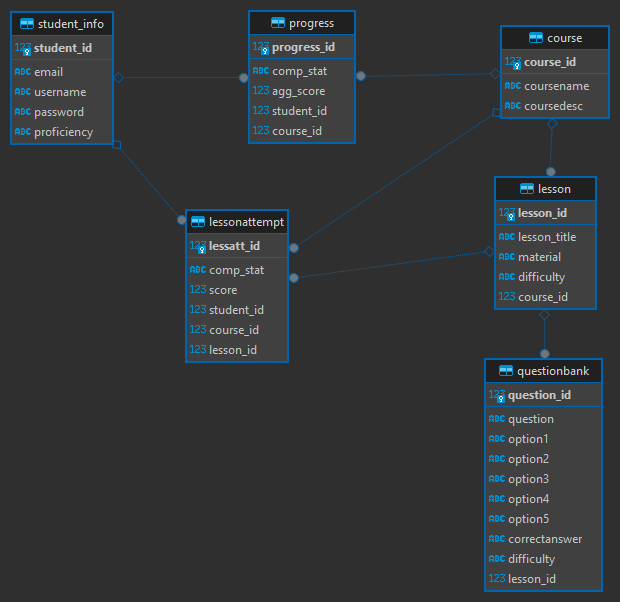
\includegraphics[width=13cm,height=9cm]{database.png}
    \caption{Database schema diagram illustrating 34 table entities and relationships}
    \label{fig:database-schema}
\end{figure}

\begin{figure}[h]
    \centering
    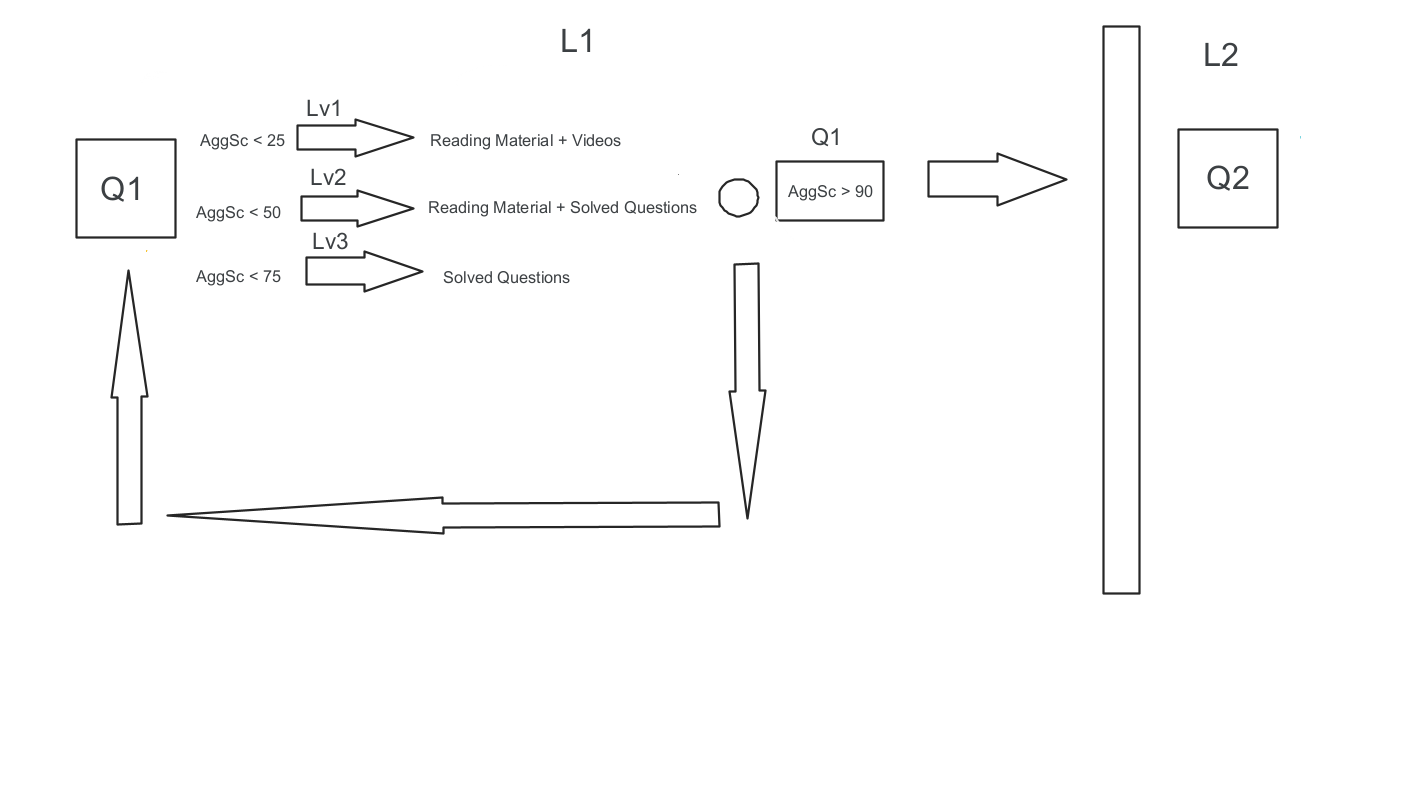
\includegraphics[width=13cm,height=9cm]{workflow.png}
    \caption{SIEM pipeline workflow from agent telemetry to dashboard visualization}
    \label{fig:pipeline-workflow}
\end{figure}